\documentclass{modernsimplecv}
% try out different fonts: classic, fira, raleway, chivo
\usepackage[utf8]{inputenc}
\usepackage[margin=1cm, a4paper]{geometry}

% ------------------------------------------------------------------------------------
% you can try out different fonts here by commenting the following lines in and out
% -----------------------------------------------------------------------------------
\usepackage[default]{raleway}
%\usepackage[sfdefault]{FiraSans} %% option 'sfdefault' activates Fira Sans as the default text font\renewcommand*\oldstylenums[1]{{\firaoldstyle #1}}\normalfont
%\usepackage[familydefault,light]{Chivo}
%\usepackage[sfdefault,light,condensed]{roboto}
%\usepackage[default]{cantarell}
%\usepackage[sfdefault]{AlegreyaSans}


\usepackage{beuron}
\usepackage{LobsterTwo}



%------------------------------------------------------------------ Variablen

\newlength{\rightcolwidth}
\newlength{\leftcolwidth}
\setlength{\leftcolwidth}{0.48\textwidth}
\setlength{\rightcolwidth}{0.47\textwidth}

%------------------------------------------------------------------
\title{Alen-resume}
\author{\LaTeX{} Ninja}
\date{August 2019}

\pagestyle{empty}
\begin{document}


\thispagestyle{empty}
%-------------------------------------------------------------



\tikz[remember picture,overlay] {%
\node[rectangle, fill=white, anchor=north, minimum width=\paperwidth, minimum height=5cm](header) at (current page.north){};%
}

\begin{minipage}[t]{0.19\textwidth}
\vspace{0pt} % Trick for alignment
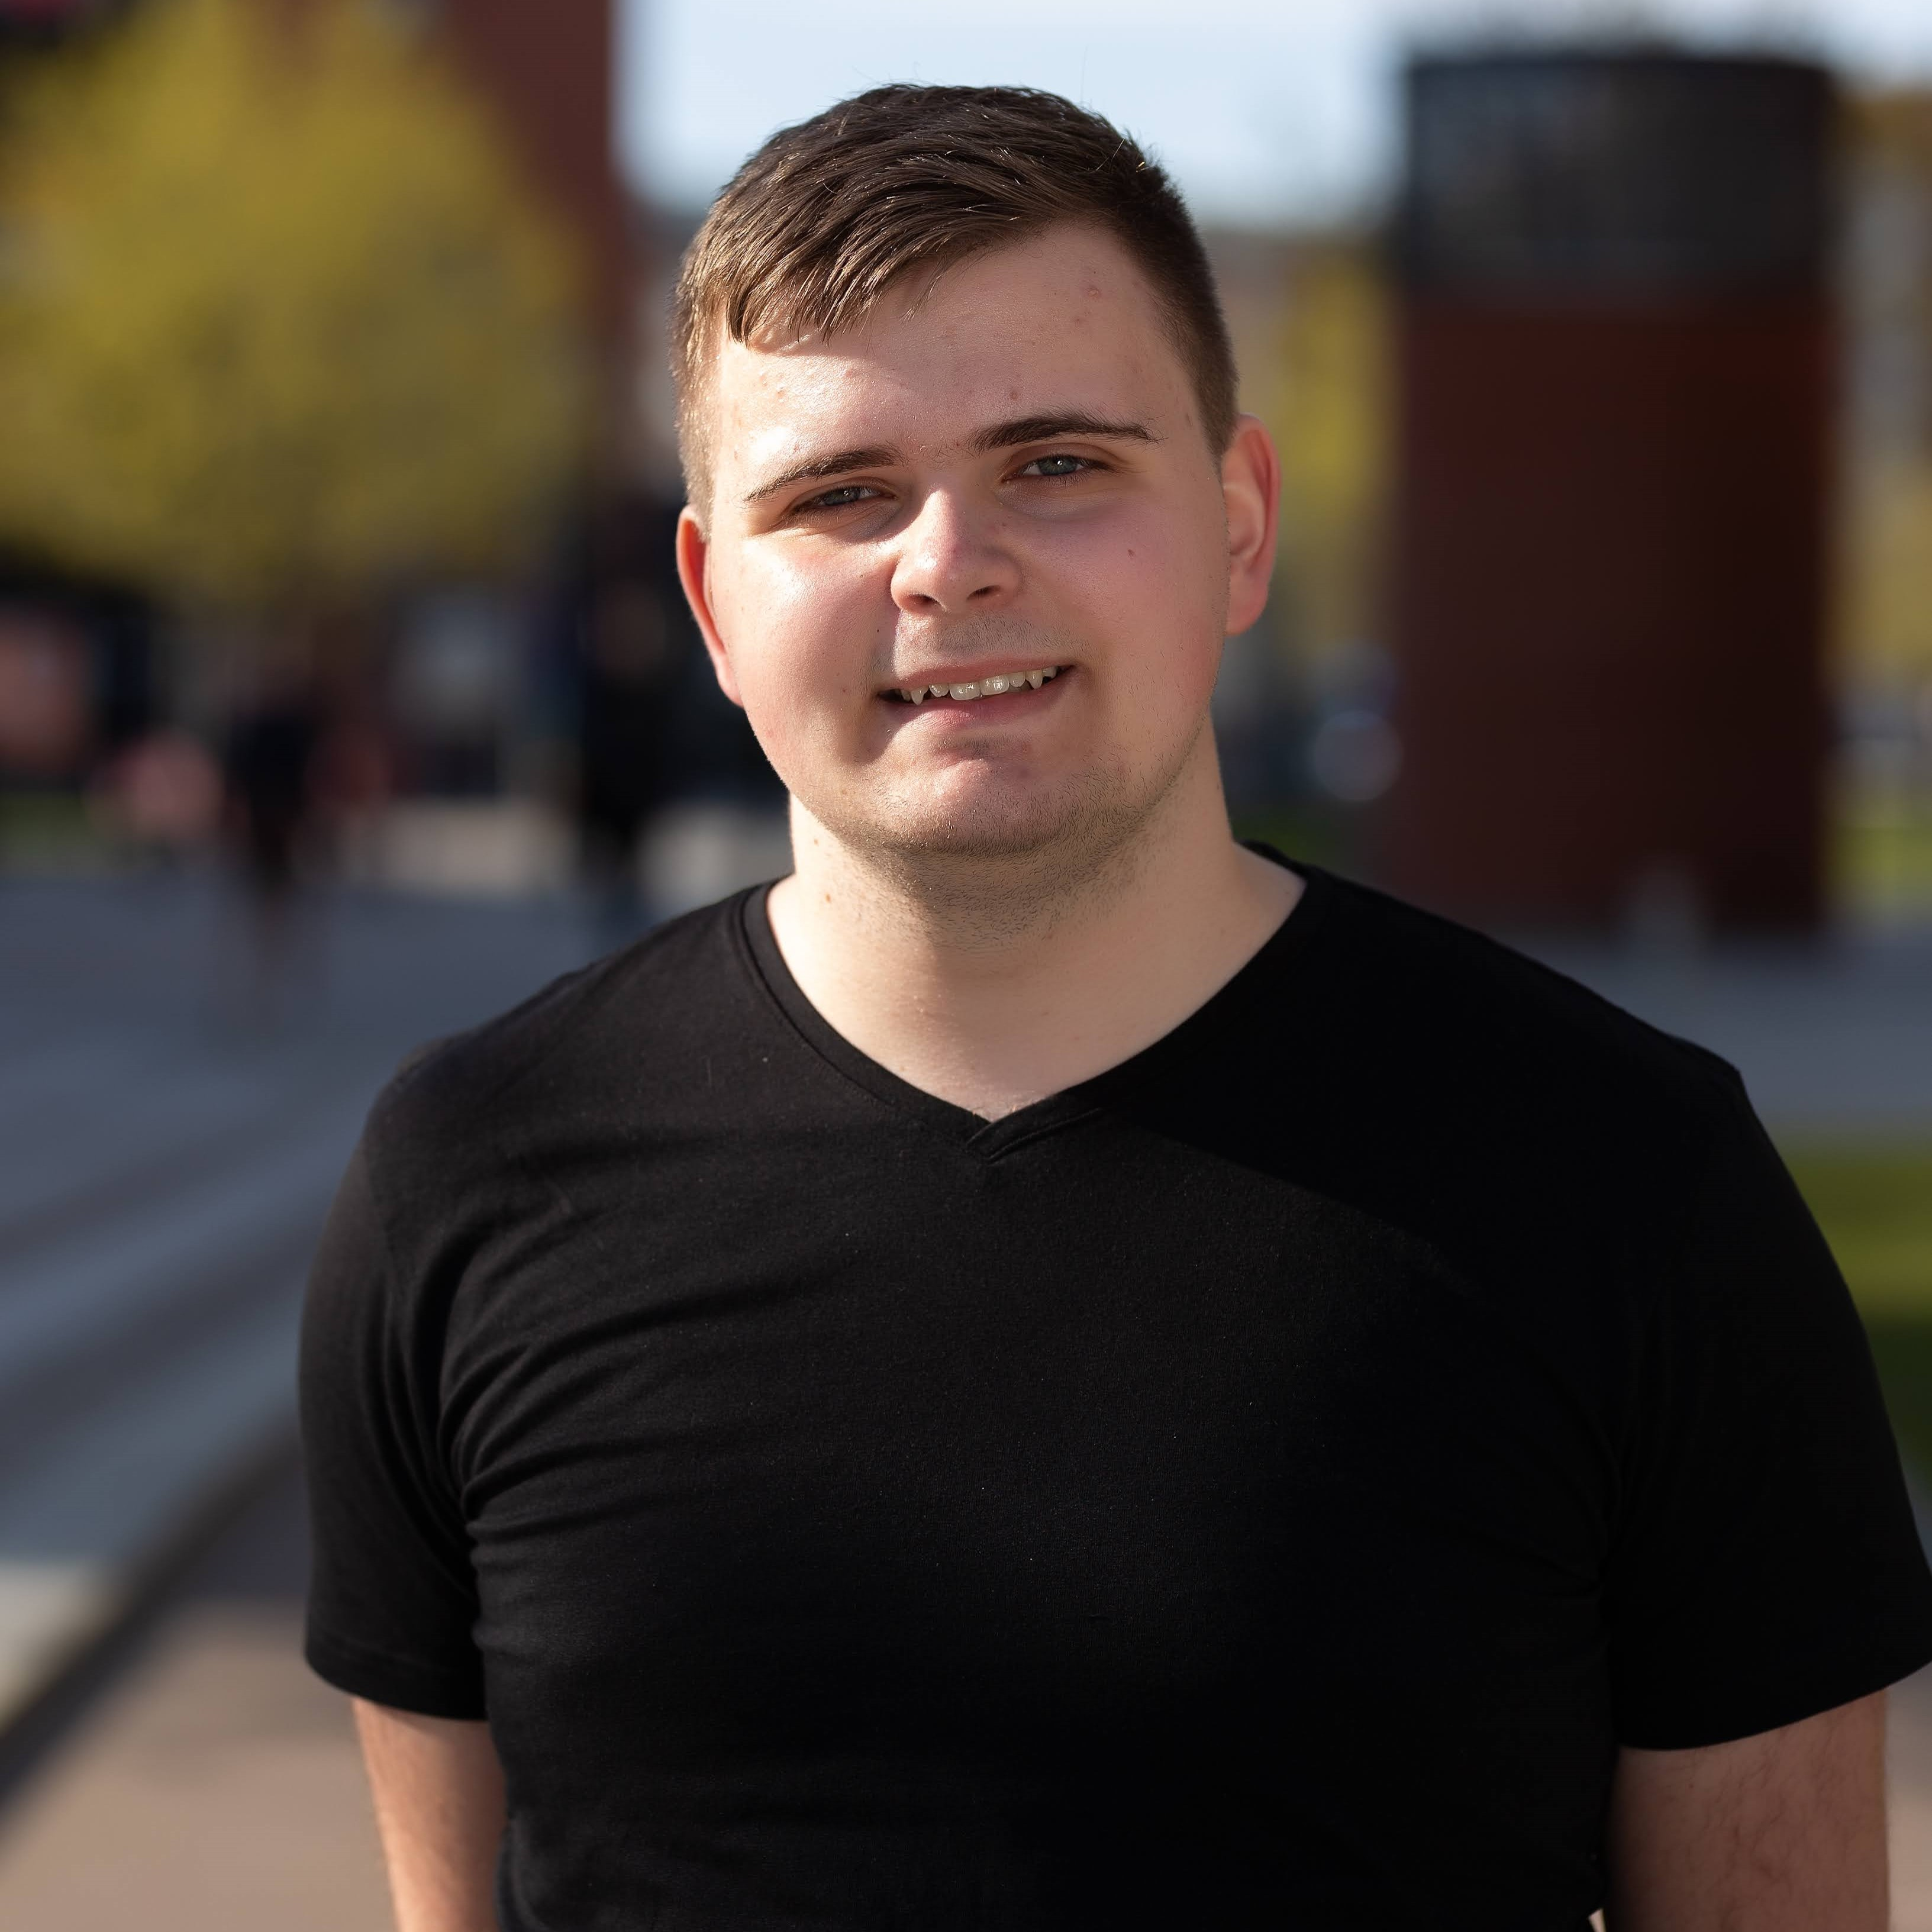
\includegraphics[width=\textwidth]{imgs/alen.jpg}\hspace{1em}
\end{minipage}
\hfill
\begin{minipage}[t]{0.8\textwidth}
\vspace{0pt} % Trick for alignment
\begin{shaded*}

\begin{minipage}[t]{0.4\textwidth}
\vspace{0pt} % Trick for alignment
% here the fancy font can be taken out by removing \LobsterTwo
{\par\centering\huge\LobsterTwo{Alen Mukaca}} \\[0.3cm]
%\faBirthdayCake~ 2001 (22) \\
%\faGlobe~ Nationality: Swedish \\

{\small
\faGraduationCap~ \underline{Title:} Cloud Developer \\
\faCommentsO~\underline{Languages:} \emph{Swedish} (Fluent C2), \\ \emph{English} (Fluent C1), \\ \emph{Bosnian} (Elementary A2).}
\end{minipage}\hfill
\begin{minipage}[t]{0.55\textwidth}
\vspace{0pt} % Trick for alignment
\href{tel:+46762160103}{\faPhone~ (+46) 762 1601013} \\
\href{mailto:alen.mukaca@gmail.com}{\faEnvelopeO~ \protect alen.mukaca@gmail.com} \\[0.1cm]

%\faMapMarker~ Gibraltargatan 80, 412 79 Gotheburg \\
%\aiAcademiaSquare
\href{https://linkedin.com/in/alen-mukaca/}{\faLinkedin~ \protect linkedin.com/in/alen-mukaca} \\
\href{https://github.com/ShinzenATT}{\faGithub~ \protect github.com/ShinzenATT} \\
\href{https://shinzle.net}{\faGlobe~ \protect www.shinzle.net}
\end{minipage}
\hfill
\end{shaded*}
\end{minipage}\\[5pt]


%------------------------------------------------

% hier muss die "unsichtbare" Überschrift rein, weil er sonst nicht die Paracols startet... komisch...
\subsection*{}
\vspace{-3em}

\setlength{\columnsep}{1.5cm}
\columnratio{0.48}[0.47]
\begin{paracol}{2}
\hbadness5000
%\backgroundcolor{c[1]}[rgb]{1,1,0.8} % cream yellow for column-1 %\backgroundcolor{g}[rgb]{0.8,1,1} % \backgroundcolor{l}[rgb]{0,0,0.7} % dark blue for left margin

\paracolbackgroundoptions

% 0.9,0.9,0.9 -- 0.8,0.8,0.8


\footnotesize
{

\small

\begin{minipage}[t]{\leftcolwidth}

\section*{Work Experience}

\begin{tabular}{p{0.2\textwidth} | p{0.6\textwidth}}
    \cvevent{Aug 2023 - Jan 2024}{Cloud/Back-end Consultant}
    {Volvo Group Connected Solutions through New Minds}{Gotheburg}{
        ...
    }{imgs/vgcs_new_minds.jpg} \\

    \cvevent{Jun - Aug 2023}{Part-time IOT Developer}{
        Combitech}{Gotheburg}{
        Interfaced a ROS based robot with an exisitng IOT platform by creating a Kotlin based middleware.
        The middleware exposes a REST api for actions and sends MQTT msgs for tracked data.
        The robot's python code hade be configured use websocket with the middleware and the middleware handled the events with coroutines.
    }{imgs/combitech.jpg} \\

    \cvevent{Jan - Jun 2023}{Bachelors Thesis - VR \& Robot}{
    Combitech}{Gotheburg}{
    Created a VR application that controls to a real-life robot wirelessly.
    The application is made in Godot and C\# that interfaces with OpenXR.
    The robot is a car with a arm that runs ROS with Python in Ubuntu.
    }{imgs/combitech.jpg}
\end{tabular}

\lineheading{125px}{Code Skills}{\faCode}{black}
\lineheading{125px}{Misc. Skills}{\faUser}{black}\\
\hspace*{10px}
\begin{skillsection}{115px}
    \cvitem{\faStar\faStar\faStar\faStar\faStar}{Java \& Kotlin}
    \cvitem{\faStar\faStar\faStar\faStar\faStarO}{Vue.js \& TypeScript}
    \cvitem{\faStar\faStar\faStar\faStar\faStarO}{Docker \& Linux}
    \cvitem{\faStar\faStar\faStar\faStarO\faStarO}{PostgreSQL}
    \cvitem{\faStar\faStar\faStarO\faStarO\faStarO}{C}
\end{skillsection}
\hspace{10px}
\begin{skillsection}{115px}
    \cvitem{\faStar\faStar\faStar\faStar\faStarO}{Planning}
    \cvitem{\faStar\faStar\faStar\faStarO\faStarO}{Teaching}
    \cvitem{\faStar\faStar\faStar\faStarO\faStarO}{(UX) Design}
    \cvitem{\faStar\faStar\faStar\faStarO\faStarO}{Image/Video Editing}
    \cvitem{\faStar\faStar\faStarO\faStarO\faStarO}{Coordination}
\end{skillsection}

\vspace{1em}

\small
\section*{Volunteering Experience}

\begin{tabular}{p{0.2\textwidth}| p{0.6\textwidth}}
    \cvevent{May 2022 - Apr 2023}{IT-Responsible and Comissioner}{Lindholmens Pubförening (PubF)}{Lindholmen, Gothenburg}{
        Managed a pub and various IT systems such as Google Workspace, DNS for email, booking system in PHP and Wordpress.
    }{imgs/pubf.png} \\
    \cvevent{Apr 2021 - Apr 2022}{Comissioner and Code Responsible}{H-Sektionens Datorförening (HD)}{Chalmers}{
        Created Vue.js websites, REST APIs in Kotlin and deployed them with Docker. Planned and hosted events. Helped students with coding.
    }{imgs/hd.png} \\
    %\cvevent{2018--2019}{Student Ambassador}{NTI Gymnasiet}{Kronhusgatan, Gothenburg}{Advertises the school by representing the school at events and fairs.}{imgs/nti.png}
\end{tabular}

%\vspace{4em}
\end{minipage}

%\begin{minipage}[t]{\leftcolwidth}
%\section*{Degrees}
%\begin{tabular}{r p{0.6\textwidth} c}
%    \cvdegree{1710}{Captain}{Certified}{Tortuga Uni}{}{disney.png} \\
%    \cvdegree{1715}{Bucaneering}{M.A.}{London}{}{medal.jpeg} \\
%    \cvdegree{1720}{Bucaneering}{B.A.}{London}{}{medal.jpeg}
%\end{tabular}
%\end{minipage}\hfill

%\vspace{3em}

%\begin{minipage}[t]{\leftcolwidth}
%\section*{Certificates \& Grants}
%\begin{tabular}{>{\footnotesize\bfseries}r >{\footnotesize}p{0.55\textwidth}}
%    1708 & Captain's Certificates \\
%    1710 & Travel grant \\
%    1715--1716 & Grant from the Pirate's Company\\
%    1708 & Captain's Certificates \\
%    1710 & Travel grant \\
%    1715--1716 & Grant from the Pirate's Company
%\end{tabular}
%\bigskip

%\end{minipage}\hfill
}
%-----------------------------------------------------------
\switchcolumn

\begin{minipage}[t]{\rightcolwidth}

\section*{Education}

\begin{tabular}{p{0.2\textwidth}| p{0.6\textwidth} c}
    \cvevent{2020--2023}{Computer Engineering, Bachelors)}{Chalmers University of Technology}{Gothenburg}{Developed with C and applied it in several ways such as embedded and concurrent programming. Also coded in Java while applying design patterns, using TCP communication, created swing UIs, and programmed concurrently. Courses also included agile SCRUM, Erlang, UX design, Requirements Engineering.}{imgs/chalmers.jpg} \\

    \cvevent{2017--2020}{High School Technology Student}{NTI Gymnasiet Kronhus}{Gothenburg}{Developed with Java and C\# whilst working with UI and SOLID. Also developed HTML, CSS \& JavaScript as well as PHP with a MySQL database. Additionally worked with Interface design and how to mock--up User Interfaces.}{imgs/nti.png} \\
\end{tabular}

\end{minipage}

\vspace{1em}

\section{Projects \& Course Projects}\label{sec:projects-&-course-projects}
\begin{tabular}{>{\footnotesize\bfseries}r >{\footnotesize}p{0.35\textwidth}}
    PubF & System Adminstration such as migrating services to Google Workspace, configuring DNS and improving booking system made in Laravel PHP and Vue.js. \vspace{3px} \\
    \href{https://www.student.chalmers.se/sp/course?course_id=34088}{DAT067} & A Radio streaming app that is made with Flutter and a Dart HTTP \& websocket server for streaming of audio. Is commissioned by LNDN AB for the course.  \vspace{3px} \\
    \href{https://www.student.chalmers.se/sp/course?course_id=33536}{DAT356} & Worked with User Experience (UX) and Requirements Engineering (RE). For RE we wrote specification and requirements while visualising them in Use-case, Context or I* Diagrams. For UX we did mock-ups and applied UI design principles. \vspace{3px} \\
    \href{https://www.student.chalmers.se/sp/course?course_id=34092}{DAT257} & While learning the agile method SCRUM we made a React TypeScript web app and a simple Java Spring Boot HTTP server for calculating emissions for a trip.\vspace{3px} \\
    \href{https://www.student.chalmers.se/sp/course?course_id=34004}{TDA384} & Covered both threaded concurrency and message passing between processes where Java and Erlang was used respectively. \vspace{3px} \\
    HD & Full-stack website with TypeScript Vue.js web app and Kotlin with Ktor HTTP API that are containerised with Docker. \vspace{3px} \\

\end{tabular}

\section{Refrences}\label{sec:refrences}
Refrences are available on request.

%\bigskip


%\begin{minipage}[t]{\rightcolwidth}
%\section*{Publications}
%\begin{tabular}{>{\footnotesize\bfseries}r >{\footnotesize}p{0.7\textwidth}}
%    1729 & \emph{How I almost got killed by Lady Swan}, Tortuga Printing Press. \\
%    1720 & ``Privateering for Beginners'', in: \emph{The Pragmatic Pirate} (1/1720).\\
%    1729 & \emph{How I almost got killed by Lady Swan}, Tortuga Printing Press. \\
%    1720 & ``Privateering for Beginners'', in: \emph{The Pragmatic Pirate} (1/1720).\\
%    1729 & \emph{How I almost got killed by Lady Swan}, Tortuga Printing Press. \\
%    1720 & ``Privateering for Beginners'', in: \emph{The Pragmatic Pirate} (1/1720).
%\end{tabular}
%\bigskip

%\section*{Talks}
%\begin{tabular}{>{\footnotesize\bfseries}r >{\footnotesize}p{0.6\textwidth}}
%    Nov. 1726 & ``How I lost my ship (\& and how to get it back)'', at: \emph{Annual Pirate's Conference} in Tortuga, Nov. 1726. \\
%    Nov. 1726 & ``How I lost my ship (\& and how to get it back)'', at: \emph{Annual Pirate's Conference} in Tortuga, Nov. 1726. \\
%    Nov. 1726 & ``How I lost my ship (\& and how to get it back)'', at: \emph{Annual Pirate's Conference} in Tortuga, Nov. 1726.
%\end{tabular}
%\end{minipage}









\end{paracol}

\vfill{} % Whitespace before final footer

%----------------------------------------------------------------------------------------
%	FINAL FOOTER
%----------------------------------------------------------------------------------------
%\setlength{\parindent}{0pt}
%\begin{minipage}[t]{\textwidth}
%\begin{center}\fontfamily{\sfdefault}\selectfont \color{black!70}
%{\small Alen Mukaca \icon{\faMapMarker}{black}{} Gibraltargatan 80, Gothenburg
%\href{tel:+46762160103}{\icon{\faPhone}{black}{} (+46) 762 160103}
%\href{mailto:alen.mukaca@gmail.com}{\icon{\faEnvelopeO}{black}{} \protect alen.mukaca@gmail.com}
%}
%\end{center}
%\end{minipage}

\end{document}
